%% This file was auto-generated by IPython.
%% Conversion from the original notebook file:
%% Exercise 7.ipynb
%%
\documentclass[a4paper, 12pt]{article}

%% This is the automatic preamble used by IPython.  Note that it does *not*
%% include a documentclass declaration. The documentclass is added at runtime
%% to the overall document.
\usepackage{fancyhdr}
\usepackage{amsmath}
\usepackage{amssymb}
\usepackage{graphicx}
\usepackage{ucs}
\usepackage[utf8x]{inputenc}

% needed for markdown enumerations to work
\usepackage{enumerate}

% Slightly bigger margins than the latex defaults
\usepackage{geometry}
\geometry{verbose,tmargin=3cm,bmargin=3cm,lmargin=2.5cm,rmargin=2.5cm}

% Define a few colors for use in code, links and cell shading
\usepackage{color}
\definecolor{orange}{cmyk}{0,0.4,0.8,0.2}
\definecolor{darkorange}{rgb}{.71,0.21,0.01}
\definecolor{darkgreen}{rgb}{.12,.54,.11}
\definecolor{myteal}{rgb}{.26, .44, .56}
\definecolor{gray}{gray}{0.45}
\definecolor{lightgray}{gray}{.95}
\definecolor{mediumgray}{gray}{.8}
\definecolor{inputbackground}{rgb}{.95, .95, .85}
\definecolor{outputbackground}{rgb}{.95, .95, .95}
\definecolor{traceback}{rgb}{1, .95, .95}

% Framed environments for code cells (inputs, outputs, errors, ...).  The
% various uses of \unskip (or not) at the end were fine-tuned by hand, so don't
% randomly change them unless you're sure of the effect it will have.
\usepackage{framed}

% remove extraneous vertical space in boxes
\setlength\fboxsep{0pt}

% codecell is the whole input+output set of blocks that a Code cell can
% generate.

% TODO: unfortunately, it seems that using a framed codecell environment breaks
% the ability of the frames inside of it to be broken across pages.  This
% causes at least the problem of having lots of empty space at the bottom of
% pages as new frames are moved to the next page, and if a single frame is too
% long to fit on a page, it will completely stop latex from compiling the
% document.  So unless we figure out a solution to this, we'll have to instead
% leave the codecell env. as empty.  I'm keeping the original codecell
% definition here (a thin vertical bar) for reference, in case we find a
% solution to the page break issue.

%% \newenvironment{codecell}{%
%%     \def\FrameCommand{\color{mediumgray} \vrule width 1pt \hspace{5pt}}%
%%    \MakeFramed{\vspace{-0.5em}}}
%%  {\unskip\endMakeFramed}

% For now, make this a no-op...
\newenvironment{codecell}{}

 \newenvironment{codeinput}{%
   \def\FrameCommand{\colorbox{inputbackground}}%
   \MakeFramed{\advance\hsize-\width \FrameRestore}}
 {\unskip\endMakeFramed}

\newenvironment{codeoutput}{%
   \def\FrameCommand{\colorbox{outputbackground}}%
   \vspace{-1.4em}
   \MakeFramed{\advance\hsize-\width \FrameRestore}}
 {\unskip\medskip\endMakeFramed}

\newenvironment{traceback}{%
   \def\FrameCommand{\colorbox{traceback}}%
   \MakeFramed{\advance\hsize-\width \FrameRestore}}
 {\endMakeFramed}

% Use and configure listings package for nicely formatted code
\usepackage{listingsutf8}
\lstset{
  language=python,
  inputencoding=utf8x,
  extendedchars=\true,
  aboveskip=\smallskipamount,
  belowskip=\smallskipamount,
  xleftmargin=2mm,
  breaklines=true,
  basicstyle=\small \ttfamily,
  showstringspaces=false,
  keywordstyle=\color{blue}\bfseries,
  commentstyle=\color{myteal},
  stringstyle=\color{darkgreen},
  identifierstyle=\color{darkorange},
  columns=fullflexible,  % tighter character kerning, like verb
}

% The hyperref package gives us a pdf with properly built
% internal navigation ('pdf bookmarks' for the table of contents,
% internal cross-reference links, web links for URLs, etc.)
\usepackage{hyperref}
\hypersetup{
  breaklinks=true,  % so long urls are correctly broken across lines
  colorlinks=true,
  urlcolor=blue,
  linkcolor=darkorange,
  citecolor=darkgreen,
  }

% hardcode size of all verbatim environments to be a bit smaller
\makeatletter
\g@addto@macro\@verbatim\small\topsep=0.5em\partopsep=0pt
\makeatother

% Prevent overflowing lines due to urls and other hard-to-break entities.
\sloppy

\newcommand{\HRule}{\rule{\linewidth}{0.5mm}}
\title{\bf Kurtosis, negentropy, and the independent components of image patches}
\author{Xugang Zhou \\ Fangzhou Yang}
\pagestyle{fancy}
\lhead{{\bf Machine Intelligence 2 SS2013}}
\rhead{Exercise 07}
\renewcommand{\headrulewidth}{0.4pt}

\begin{document}
\begin{titlepage}
\begin{center}
\vfill
\textsc{\LARGE Machine Intelligence 2}\\[1.5cm]
\textsc{\Large Exercise 07}\\[0.5cm]

\HRule \\[0.4cm]
{\huge \bfseries Kurtosis, negentropy, and the independent components of image patches}\\[0.4cm]
\HRule \\[1.5cm]
\begin{minipage}{0.4\textwidth}
\begin{flushleft} \large
\emph{Group Members:}\\
Xugang \textsc{Zhou}\\
Fangzhou \textsc{Yang}
\end{flushleft}
\end{minipage}
\begin{minipage}{0.4\textwidth}
\begin{flushright} \large
\emph{Tutor:} \\
Timm \textsc{Lochmann} \\
\end{flushright}
\end{minipage}
\vfill
{\large \today}\\
\end{center}
\end{titlepage}
\thispagestyle{fancy}


\section{7.1 Kurtosis of Toy Data}

\begin{codecell}
\begin{codeinput}
\begin{lstlisting}
from numpy import *
from scipy import linalg, io
from scipy.linalg import sqrtm, inv
from scipy.io import loadmat
import matplotlib
import matplotlib.pyplot as plt
from PrincipalComponentsTool import get_PC
from math import *

def plotSaH(X, Y, Name, c, ran):
    fig = plt.figure()
    plt.suptitle(Name)
    ax = plt.subplot2grid((2, 3), (0, 0), rowspan = 2, colspan = 2)
    ax.axis([-ran, ran, -ran, ran])
    ax.plot(X, Y, c + '.')
    ax = plt.subplot2grid((2, 3), (0, 2))
    ax.hist(X, 50, normed = 1, facecolor = c, alpha = 0.75)
    ax.set_xlabel("1st Dimension")
    ax = plt.subplot2grid((2, 3), (1, 2))
    ax.hist(Y, 50, normed = 1, facecolor = c, alpha = 0.75)
    ax.set_xlabel("2nd Dimension")
    #fig.savefig(Name+".png")


\end{lstlisting}
\end{codeinput}
\end{codecell}
\begin{codecell}
\begin{codeinput}
\begin{lstlisting}
matData = loadmat("datafilesICA/distrib.mat")

dic = ["normal", "laplacian", "uniform"]
color = ['b', 'r', 'g']

data = [0 for i in range(3)]
A = [[4, 3],[1, 2]]
for i in range(3):
    data[i] = matData[dic[i]]
    plotSaH(data[i][0], data[i][1], "Original Data " + dic[i], color[i], 20)
\end{lstlisting}
\end{codeinput}
\begin{codeoutput}
\begin{center}
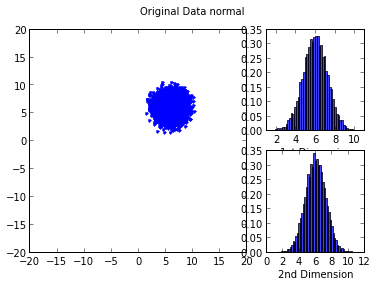
\includegraphics[width=0.7\textwidth]{Exercise_7_files/Exercise_7_fig_00.png}
\par
\end{center}
\begin{center}
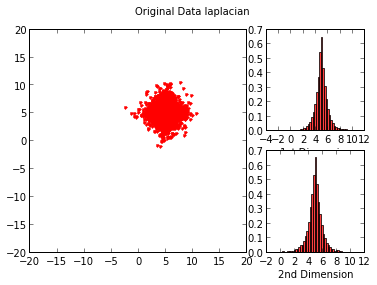
\includegraphics[width=0.7\textwidth]{Exercise_7_files/Exercise_7_fig_01.png}
\par
\end{center}
\begin{center}
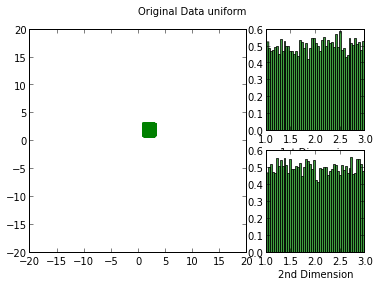
\includegraphics[width=0.7\textwidth]{Exercise_7_files/Exercise_7_fig_02.png}
\par
\end{center}
\end{codeoutput}
\end{codecell}
\begin{codecell}
\begin{codeinput}
\begin{lstlisting}
mixed = [0 for i in range(3)]
for i in range(3):
    mixed[i] = [[sum(A[j][k] * data[i][k][l] for k in range(2)) for l in range(10000)] for j in range(2)]
    m0 = sum(mixed[i][0]) / 10000
    m1 = sum(mixed[i][1]) / 10000
    mixed[i][0] = [mixed[i][0][j] - m0 for j in range(10000)]
    mixed[i][1] = [mixed[i][1][j] - m1 for j in range(10000)]
    plotSaH(mixed[i][0], mixed[i][1], "Centered Mix " + dic[i], color[i], 30)
\end{lstlisting}
\end{codeinput}
\begin{codeoutput}
\begin{center}
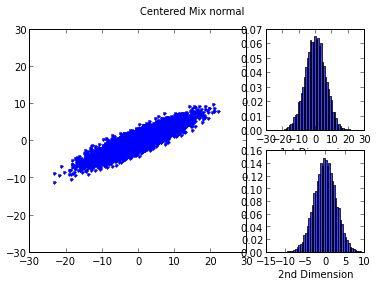
\includegraphics[width=0.7\textwidth]{Exercise_7_files/Exercise_7_fig_03.png}
\par
\end{center}
\begin{center}
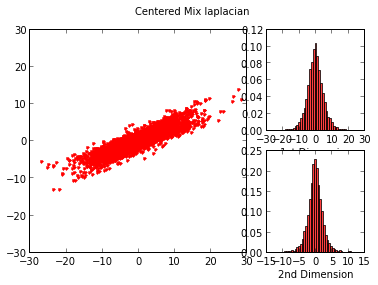
\includegraphics[width=0.7\textwidth]{Exercise_7_files/Exercise_7_fig_04.png}
\par
\end{center}
\begin{center}
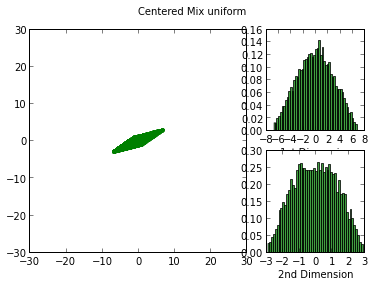
\includegraphics[width=0.7\textwidth]{Exercise_7_files/Exercise_7_fig_05.png}
\par
\end{center}
\end{codeoutput}
\end{codecell}
\begin{codecell}
\begin{codeinput}
\begin{lstlisting}
projected = [[0 for i in range(2)] for j in range(3)]
whiten = [0 for j in range(3)]
for i in range(3):
    evals, evecs = get_PC(mixed[i], 2, 2)
    projected[i][0] = [mixed[i][0][j] * evecs[0, 0] + mixed[i][1][j] * evecs[1, 0] for j in range(10000)]
    projected[i][1] = [mixed[i][0][j] * evecs[0, 1] + mixed[i][1][j] * evecs[1, 1] for j in range(10000)]
    plotSaH(projected[i][0], projected[i][1], "PC_Projected " + dic[i], color[i], 30)
    whiten[i] = dot(dot(array(mixed[i]).T, array(evecs)), inv(sqrtm(diag(evals))).real).T
    
    
\end{lstlisting}
\end{codeinput}
\begin{codeoutput}
\begin{center}
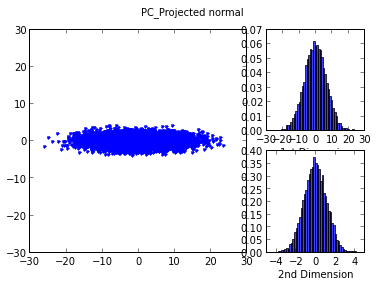
\includegraphics[width=0.7\textwidth]{Exercise_7_files/Exercise_7_fig_06.png}
\par
\end{center}
\begin{center}
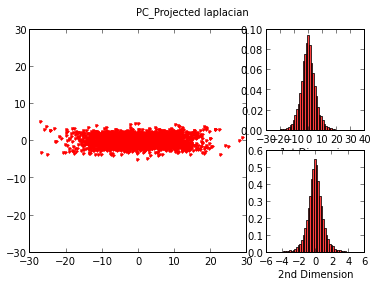
\includegraphics[width=0.7\textwidth]{Exercise_7_files/Exercise_7_fig_07.png}
\par
\end{center}
\begin{center}
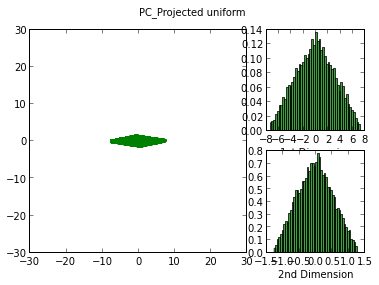
\includegraphics[width=0.7\textwidth]{Exercise_7_files/Exercise_7_fig_08.png}
\par
\end{center}
\end{codeoutput}
\end{codecell}
\begin{codecell}
\begin{codeinput}
\begin{lstlisting}
for i in range(3):
    plotSaH(whiten[i][0], whiten[i][1], "Whitened " + dic[i], color[i], 8)
\end{lstlisting}
\end{codeinput}
\begin{codeoutput}
\begin{center}
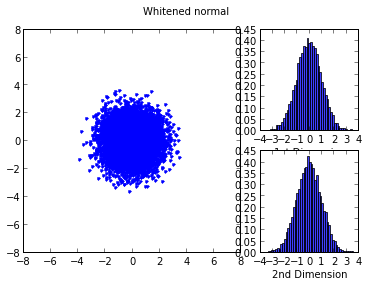
\includegraphics[width=0.7\textwidth]{Exercise_7_files/Exercise_7_fig_09.png}
\par
\end{center}
\begin{center}
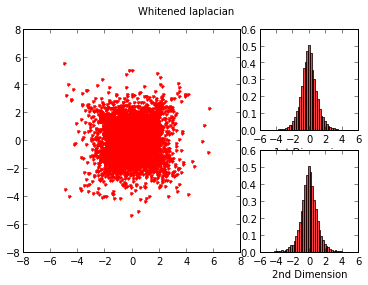
\includegraphics[width=0.7\textwidth]{Exercise_7_files/Exercise_7_fig_10.png}
\par
\end{center}
\begin{center}
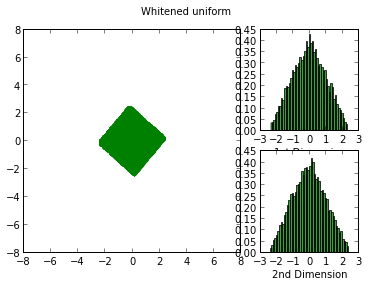
\includegraphics[width=0.7\textwidth]{Exercise_7_files/Exercise_7_fig_11.png}
\par
\end{center}
\end{codeoutput}
\end{codecell}
\begin{codecell}
\begin{codeinput}
\begin{lstlisting}
theta = [i * pi / 50 for i in range(100)]
kurtVal1 = [0 for i in range(100)]
kurtVal2 = [0 for i in range(100)]
maxData = matrix([[0 for i in range(10000)] for j in range(2)])
minData = matrix([[0 for i in range(10000)] for j in range(2)])
for i in range(3):
    minKurt = 10000
    maxKurt = -10000
    for k in range(100):
        R = array([[cos(theta[k]), -sin(theta[k])],[sin(theta[k]), cos(theta[k])]])
        tempData = dot(R, whiten[i])
        kurtVal1[k] = 0
        kurtVal2[k] = 0
        for j in range(10000):
            kurtVal1[k] += tempData[0, j] ** 4
            kurtVal2[k] += tempData[1, j] ** 4
        kurtVal1[k] = abs(kurtVal1[k] / 10000 - 3)
        kurtVal2[k] = abs(kurtVal2[k] / 10000 - 3)
        if kurtVal1[k] > maxKurt:
            maxKurt = kurtVal1[k]
            maxData = tempData
        if kurtVal1[k] < minKurt:
            minKurt = kurtVal1[k]
            minData = tempData
    plotSaH(minData[0, :], minData[1, :], "MinKurt " + dic[i], color[i], 8)
    plotSaH(maxData[0, :], maxData[1, :], "MaxKurt " + dic[i], color[i], 8)
    fig = plt.figure()
    ax = fig.add_subplot(111)
    ax.plot(theta, kurtVal1, color[i] + '-')
    ax.set_title("KurtVal 1st " + dic[i])
    fig.savefig("KurtVal 1st " + dic[i] + ".png")
    fig = plt.figure()
    ax = fig.add_subplot(111)
    ax.plot(theta, kurtVal2, color[i] + '-')
    ax.set_title("KurtVal 2nd " + dic[i])
    fig.savefig("KurtVal 2nd " + dic[i] + ".png")

\end{lstlisting}
\end{codeinput}
\begin{codeoutput}
\begin{center}
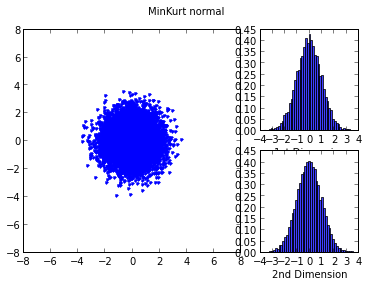
\includegraphics[width=0.7\textwidth]{Exercise_7_files/Exercise_7_fig_12.png}
\par
\end{center}
\begin{center}
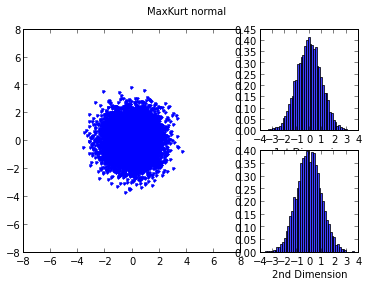
\includegraphics[width=0.7\textwidth]{Exercise_7_files/Exercise_7_fig_13.png}
\par
\end{center}
\begin{center}
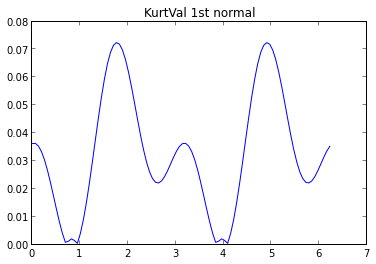
\includegraphics[width=0.7\textwidth]{Exercise_7_files/Exercise_7_fig_14.png}
\par
\end{center}
\begin{center}
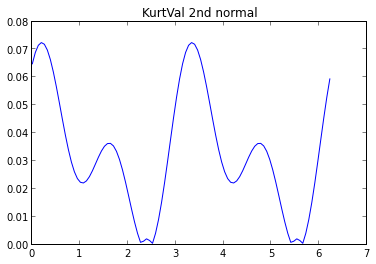
\includegraphics[width=0.7\textwidth]{Exercise_7_files/Exercise_7_fig_15.png}
\par
\end{center}
\begin{center}
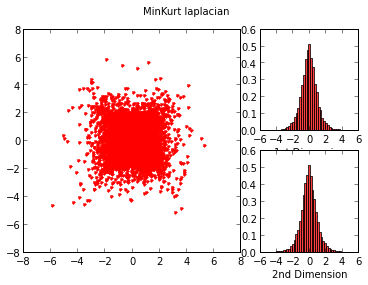
\includegraphics[width=0.7\textwidth]{Exercise_7_files/Exercise_7_fig_16.png}
\par
\end{center}
\begin{center}
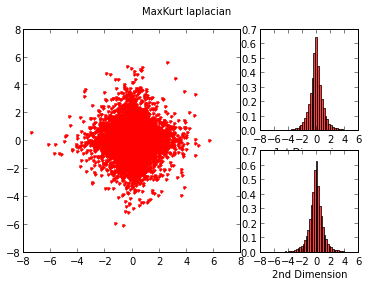
\includegraphics[width=0.7\textwidth]{Exercise_7_files/Exercise_7_fig_17.png}
\par
\end{center}
\begin{center}
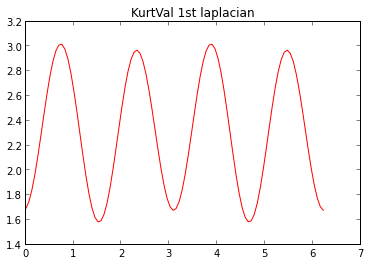
\includegraphics[width=0.7\textwidth]{Exercise_7_files/Exercise_7_fig_18.png}
\par
\end{center}
\begin{center}
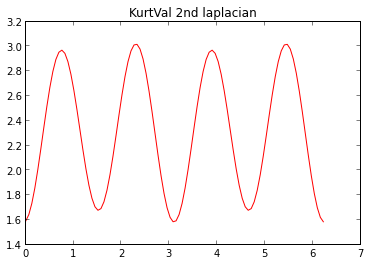
\includegraphics[width=0.7\textwidth]{Exercise_7_files/Exercise_7_fig_19.png}
\par
\end{center}
\begin{center}
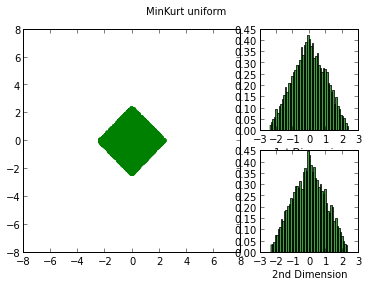
\includegraphics[width=0.7\textwidth]{Exercise_7_files/Exercise_7_fig_20.png}
\par
\end{center}
\begin{center}
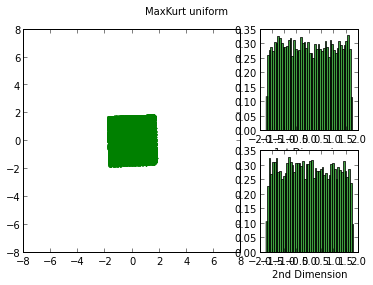
\includegraphics[width=0.7\textwidth]{Exercise_7_files/Exercise_7_fig_21.png}
\par
\end{center}
\begin{center}
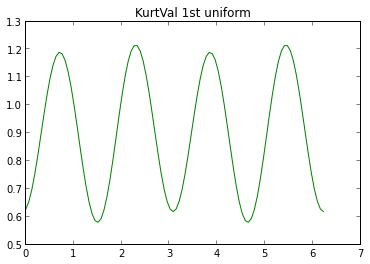
\includegraphics[width=0.7\textwidth]{Exercise_7_files/Exercise_7_fig_22.png}
\par
\end{center}
\begin{center}
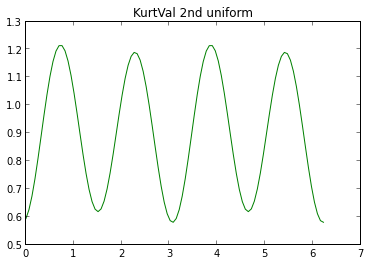
\includegraphics[width=0.7\textwidth]{Exercise_7_files/Exercise_7_fig_23.png}
\par
\end{center}
\end{codeoutput}
\end{codecell}
\section{7.2 Toy Singal Seperation}

\begin{codecell}
\begin{codeinput}
\begin{lstlisting}
xaxis = [i * 0.05 for i in range(1000)]

def plotSig(X, Name, c, ran):
    fig = plt.figure()
    ax = fig.add_subplot(111)
    ax.plot(xaxis, X, c + '-')
    ax.set_title(Name)
    ax.axis([0, 50, -ran, ran])
    #fig.savefig(Name + ".png")
\end{lstlisting}
\end{codeinput}
\end{codecell}
\begin{codecell}
\begin{codeinput}
\begin{lstlisting}
color = ['b', 'r', 'g']
s = [0 for i in range (3)]
s[0] = [4 * sin(i * 0.05 - 3) for i in range(1000)]
s[1] = [(i * 0.05 + 5) % 10 for i in range(1000)]
s[2] = [(-14 if cos(2 * 0.05 * i) > 0 else 0) for i in range(1000)]
\end{lstlisting}
\end{codeinput}
\end{codecell}
\begin{codecell}
\begin{codeinput}
\begin{lstlisting}
for i in range(3):
    plotSig(s[i], "Source " + str(i), color[i], 14)

A = array([[2, -3, -4], [7, 5, 1], [-4, 7, 5]])
x = dot(A , s)
\end{lstlisting}
\end{codeinput}
\begin{codeoutput}
\begin{center}
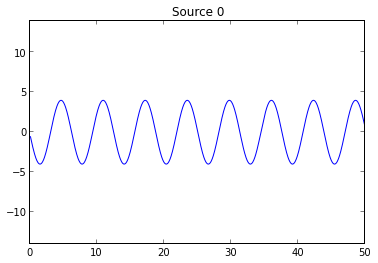
\includegraphics[width=0.7\textwidth]{Exercise_7_files/Exercise_7_fig_24.png}
\par
\end{center}
\begin{center}
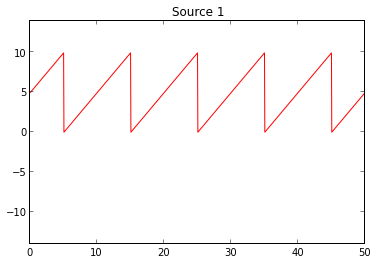
\includegraphics[width=0.7\textwidth]{Exercise_7_files/Exercise_7_fig_25.png}
\par
\end{center}
\begin{center}
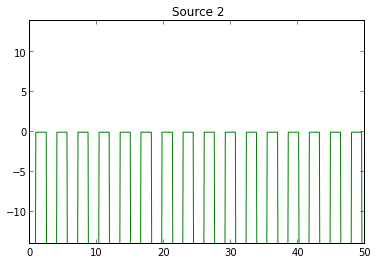
\includegraphics[width=0.7\textwidth]{Exercise_7_files/Exercise_7_fig_26.png}
\par
\end{center}
\end{codeoutput}
\end{codecell}
\begin{codecell}
\begin{codeinput}
\begin{lstlisting}
for i in range(3):
    plotSig(x[i, :], "Mixed " + str(i), color[i], 100)
\end{lstlisting}
\end{codeinput}
\begin{codeoutput}
\begin{center}
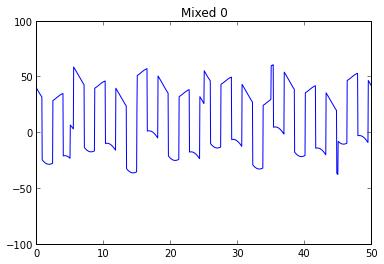
\includegraphics[width=0.7\textwidth]{Exercise_7_files/Exercise_7_fig_27.png}
\par
\end{center}
\begin{center}
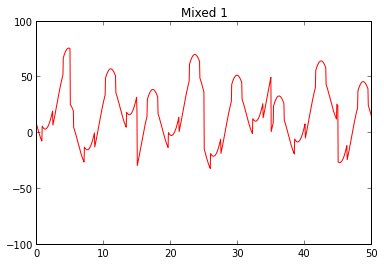
\includegraphics[width=0.7\textwidth]{Exercise_7_files/Exercise_7_fig_28.png}
\par
\end{center}
\begin{center}
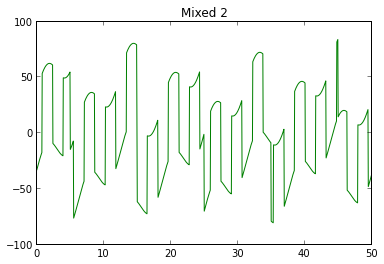
\includegraphics[width=0.7\textwidth]{Exercise_7_files/Exercise_7_fig_29.png}
\par
\end{center}
\end{codeoutput}
\end{codecell}
\begin{codecell}
\begin{codeinput}
\begin{lstlisting}
evals, evecs = get_PC(x, 3, 3)
whiten = dot(dot(x.T, array(evecs)), inv(sqrtm(diag(evals))).real).T
for i in range(3):
    plotSig(whiten[i, :], "Whiten " + str(i), color[i], 5)

\end{lstlisting}
\end{codeinput}
\begin{codeoutput}
\begin{center}
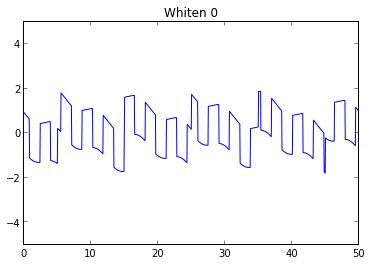
\includegraphics[width=0.7\textwidth]{Exercise_7_files/Exercise_7_fig_30.png}
\par
\end{center}
\begin{center}
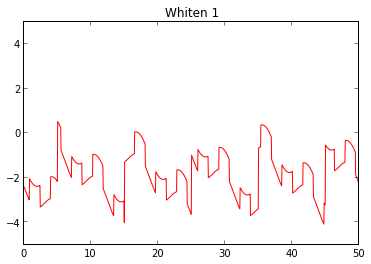
\includegraphics[width=0.7\textwidth]{Exercise_7_files/Exercise_7_fig_31.png}
\par
\end{center}
\begin{center}
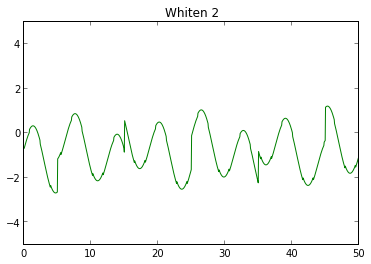
\includegraphics[width=0.7\textwidth]{Exercise_7_files/Exercise_7_fig_32.png}
\par
\end{center}
\end{codeoutput}
\end{codecell}
\begin{codecell}
\begin{codeinput}
\begin{lstlisting}
import mdp
y = mdp.fastica(whiten.T, g = 'pow3').T
for i in range(3):
    plotSig(y[i, :], "Unmixed_pow3 " + str(i), color[i], 2)
\end{lstlisting}
\end{codeinput}
\begin{codeoutput}
\begin{center}
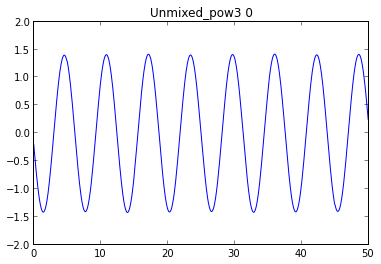
\includegraphics[width=0.7\textwidth]{Exercise_7_files/Exercise_7_fig_33.png}
\par
\end{center}
\begin{center}
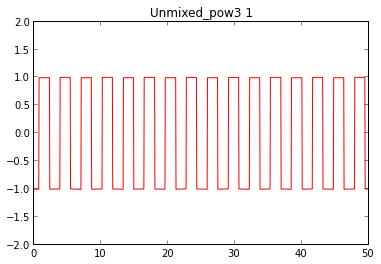
\includegraphics[width=0.7\textwidth]{Exercise_7_files/Exercise_7_fig_34.png}
\par
\end{center}
\begin{center}
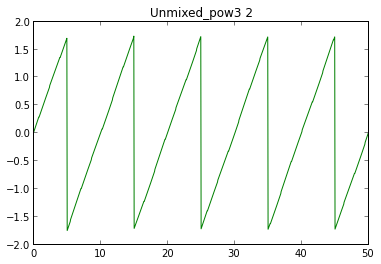
\includegraphics[width=0.7\textwidth]{Exercise_7_files/Exercise_7_fig_35.png}
\par
\end{center}
\end{codeoutput}
\end{codecell}
\begin{codecell}
\begin{codeinput}
\begin{lstlisting}
y = mdp.fastica(whiten.T, g='tanh').T
for i in range(3):
    plotSig(y[i, :], "Unmixed_tanh " + str(i), color[i], 2)
\end{lstlisting}
\end{codeinput}
\begin{codeoutput}
\begin{center}
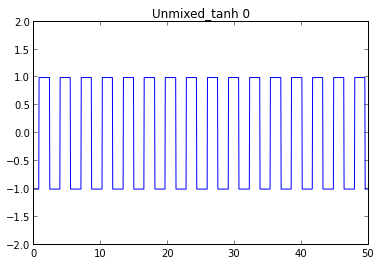
\includegraphics[width=0.7\textwidth]{Exercise_7_files/Exercise_7_fig_36.png}
\par
\end{center}
\begin{center}
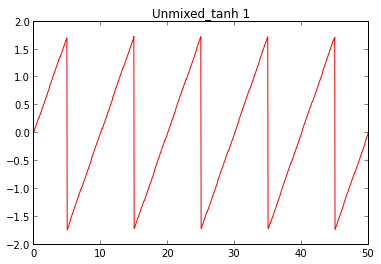
\includegraphics[width=0.7\textwidth]{Exercise_7_files/Exercise_7_fig_37.png}
\par
\end{center}
\begin{center}
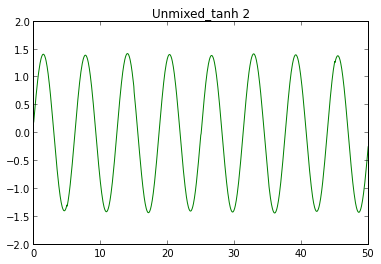
\includegraphics[width=0.7\textwidth]{Exercise_7_files/Exercise_7_fig_38.png}
\par
\end{center}
\end{codeoutput}
\end{codecell}
\section{7.3 ICA on Image Patches}

\begin{codecell}
\begin{codeinput}
\begin{lstlisting}
from mahotas import imread
from numpy import *

N = 16
numP = 2000

buildingData = [[] for i in range(10 * numP)]
for i in range(10):
    readImage = imread('datafilesICA/images/b'+str(i+1)+'.jpg')
    for j in range(numP):
        startPosx = random.randint(0, readImage.shape[0] - N - 1)
        startPosy = random.randint(0, readImage.shape[1] - N - 1)
        sample = readImage[startPosx:startPosx + N, startPosy:startPosy + N]
        buildingData[i * numP + j] = [x for sublist in sample for x in sublist]

savetxt('buildingData', buildingData)

natureData = [[] for i in range(13 * numP)]
for i in range(13):
    readImage = imread('datafilesICA/images/n'+str(i+1)+'.jpg')
    for j in range(numP):
        startPosx = random.randint(0, readImage.shape[0] - N - 1)
        startPosy = random.randint(0, readImage.shape[1] - N - 1)
        sample = readImage[startPosx:startPosx + N, startPosy:startPosy + N]
        natureData[i * numP + j] = [x for sublist in sample for x in sublist]

savetxt('natureData', natureData)

textData = [[] for i in range(14 * numP)]
for i in range(14):
    readImage = imread('datafilesICA/images/t'+str(i+1)+'.jpg')
    for j in range(numP):
        startPosx = random.randint(0, readImage.shape[0] - N - 1)
        startPosy = random.randint(0, readImage.shape[1] - N - 1)
        sample = readImage[startPosx:startPosx + N, startPosy:startPosy + N]
        textData[i * numP + j] = [x for sublist in sample for x in sublist]

savetxt('textData', textData)
\end{lstlisting}
\end{codeinput}
\end{codecell}
\begin{codecell}
\begin{codeinput}
\begin{lstlisting}
from sklearn.decomposition import FastICA
dic = ["building", "nature", "text"]
color = ['b', 'r', 'g']
for i in range(3):
    print "Processing " + dic[i]
    data = loadtxt(dic[i] + "Data")
    ica = FastICA()
    output = ica.fit(data).transform(data)
    features = ica.get_mixing_matrix()
    print features.shape
    savetxt(dic[i] + "feature", features)
\end{lstlisting}
\end{codeinput}
\begin{codeoutput}
\begin{verbatim}
Processing building
(256, 256)
\end{verbatim}
\begin{verbatim}
Processing nature
\end{verbatim}
\begin{verbatim}
(256, 256)
\end{verbatim}
\begin{verbatim}
Processing text
\end{verbatim}
\begin{verbatim}
(256, 256)
\end{verbatim}
\begin{verbatim}

\end{verbatim}
\end{codeoutput}
\end{codecell}
\begin{codecell}
\begin{codeinput}
\begin{lstlisting}
from mahotas import imsave
dic = ["building", "nature", "text"]

N = 16
img = array([[0 for i in range(N)] for j in range(N)])
for i in range(3):
    data = loadtxt(dic[i] + "feature").T
    for j in range(20):
        maxV = 0
        for a in range(N):
            for b in range(N):
                if data[j][a * N + b] > maxV:
                    maxV = data[j][a * N + b]
        for a in range(N):
            for b in range(N):
                img[a][b] = data[j][a * N + b] / maxV * 256
        imsave(dic[i] + str(j) + "_patch.jpg", img.astype(uint8))
\end{lstlisting}
\end{codeinput}
\end{codecell}
\begin{center}\rule{3in}{0.4pt}\end{center}

\subsection{Building Features:}
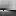
\includegraphics[width=0.18\textwidth]{building0_patch.jpg}
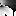
\includegraphics[width=0.18\textwidth]{building1_patch.jpg}
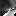
\includegraphics[width=0.18\textwidth]{building2_patch.jpg}
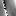
\includegraphics[width=0.18\textwidth]{building3_patch.jpg}
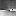
\includegraphics[width=0.18\textwidth]{building4_patch.jpg}
\newline
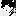
\includegraphics[width=0.18\textwidth]{building5_patch.jpg}

\includegraphics[width=0.18\textwidth]{building6_patch.jpg}
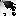
\includegraphics[width=0.18\textwidth]{building7_patch.jpg}
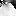
\includegraphics[width=0.18\textwidth]{building8_patch.jpg}
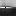
\includegraphics[width=0.18\textwidth]{building9_patch.jpg}
\newline
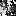
\includegraphics[width=0.18\textwidth]{building10_patch.jpg}
\includegraphics[width=0.18\textwidth]{building11_patch.jpg}
\includegraphics[width=0.18\textwidth]{building12_patch.jpg}
\includegraphics[width=0.18\textwidth]{building13_patch.jpg}
\includegraphics[width=0.18\textwidth]{building14_patch.jpg}
\newline
\includegraphics[width=0.18\textwidth]{building15_patch.jpg}
\includegraphics[width=0.18\textwidth]{building16_patch.jpg}
\includegraphics[width=0.18\textwidth]{building17_patch.jpg}
\includegraphics[width=0.18\textwidth]{building18_patch.jpg}
\includegraphics[width=0.18\textwidth]{building19_patch.jpg}
\newline
\subsection{Nature Featrues:} 
\includegraphics[width=0.18\textwidth]{nature0_patch.jpg}
\includegraphics[width=0.18\textwidth]{nature1_patch.jpg}
\includegraphics[width=0.18\textwidth]{nature2_patch.jpg}
\includegraphics[width=0.18\textwidth]{nature3_patch.jpg}
\includegraphics[width=0.18\textwidth]{nature4_patch.jpg}
\newline
\includegraphics[width=0.18\textwidth]{nature5_patch.jpg}
\includegraphics[width=0.18\textwidth]{nature6_patch.jpg}
\includegraphics[width=0.18\textwidth]{nature7_patch.jpg}
\includegraphics[width=0.18\textwidth]{nature8_patch.jpg}
\includegraphics[width=0.18\textwidth]{nature9_patch.jpg}
\newline
\includegraphics[width=0.18\textwidth]{nature10_patch.jpg}
\includegraphics[width=0.18\textwidth]{nature11_patch.jpg}
\includegraphics[width=0.18\textwidth]{nature12_patch.jpg}
\includegraphics[width=0.18\textwidth]{nature13_patch.jpg}
\includegraphics[width=0.18\textwidth]{nature14_patch.jpg}
\newline
\includegraphics[width=0.18\textwidth]{nature15_patch.jpg}
\includegraphics[width=0.18\textwidth]{nature16_patch.jpg}
\includegraphics[width=0.18\textwidth]{nature17_patch.jpg}
\includegraphics[width=0.18\textwidth]{nature18_patch.jpg}
\includegraphics[width=0.18\textwidth]{nature19_patch.jpg}
\newline
\subsection{Text Features:}
\includegraphics[width=0.18\textwidth]{text0_patch.jpg}
\includegraphics[width=0.18\textwidth]{text1_patch.jpg}
\includegraphics[width=0.18\textwidth]{text2_patch.jpg}
\includegraphics[width=0.18\textwidth]{text3_patch.jpg}
\includegraphics[width=0.18\textwidth]{text4_patch.jpg}
\newline
\includegraphics[width=0.18\textwidth]{text5_patch.jpg}
\includegraphics[width=0.18\textwidth]{text6_patch.jpg}
\includegraphics[width=0.18\textwidth]{text7_patch.jpg}
\includegraphics[width=0.18\textwidth]{text8_patch.jpg}
\includegraphics[width=0.18\textwidth]{text9_patch.jpg}
\newline
\includegraphics[width=0.18\textwidth]{text10_patch.jpg}
\includegraphics[width=0.18\textwidth]{text11_patch.jpg}
\includegraphics[width=0.18\textwidth]{text12_patch.jpg}
\includegraphics[width=0.18\textwidth]{text13_patch.jpg}
\includegraphics[width=0.18\textwidth]{text14_patch.jpg}
\newline
\includegraphics[width=0.18\textwidth]{text15_patch.jpg}
\includegraphics[width=0.18\textwidth]{text16_patch.jpg}
\includegraphics[width=0.18\textwidth]{text17_patch.jpg}
\includegraphics[width=0.18\textwidth]{text18_patch.jpg}
\includegraphics[width=0.18\textwidth]{text19_patch.jpg}
\newline
\end{document}
